\chapter{Smitc solver -- 2D -- Eigenmodes of an elastic plate}

\modinfo{Directory}{ElasticPlateEigenmodesGUI}
\modinfo{Solvers}{\Idx{SmitcSolver}} 
\modinfo{Tools}{\Idx{ElmerGUI}} 
\modinfo{Dimensions}{2D, Eigenmode}
\modinfo{Author}{Peter R{\aa}back}


\subsection*{Problem description}

For thin elastic structures it is often advisable to use dimensionally reduced models i.e. 
study plates or shells. In this tutorial we compute the few lowest eigenmodes of an elastic plate. 
Our geometry is a simple pentagon which (compared to a square) eliminates some of the trivial symmetries.
The pentagon is rigidly fixed at all boundaries.

For more details on the solver we refer to the documentation of Smitc solver in the 
Elmer Models Manual.

\subsection*{Solution procedure}

Start \texttt{ElmerGUI} from command line or by clicking the icon in your desktop. Here we describe 
the essential steps in the ElmerGUI by writing out the clicking procedure. Tabulation generally means that the 
selections are done within the window chosen at the higher level. 

Before we can start the set-up we should make sure that the menus for Smitc solver are present.
If not, they may be found in file
\ttbegin
$ELMERHOME/bin/edf-extra/elasticplate.xml
\ttend
To load these definitions do the following
\ttbegin
File
  Definitions
    Append -> choose the file
\ttend
To see what kind of new menu structures were loaded you may play around with viewer collapsing and opening. 
Note that if you want to load an existing project you should load the xml-definitions that were used 
in creating the project. Therefore it may be best to place all actively used menu definitions in
directory
\ttbegin
$ELMERHOME/bin/edf
\ttend

When the menu structures for plate solver are there then we are ready to continue.
The mesh is given in 2d netgen format in file \texttt{pentagon.grd} in the samples directory of ElmerGUI, 
load this file.
\ttbegin
File 
  Open -> pentagon.in2d
\ttend
You should obtain a pentagon consisting of 5 triangles. To increase the number of elements 
change the parameters passed on to the nglib library by going to
\ttbegin
Mesh 
  Configure
    nglib / Max H: 0.05
\ttend
You may check in the \texttt{Model summary} 
window that it consists of 1199 nodes and 2276 linear triangles.
If the mesh was successfully imported your window should look something in figure~\ref{fg:pentagonmesh}.

\begin{figure}
\begin{center}
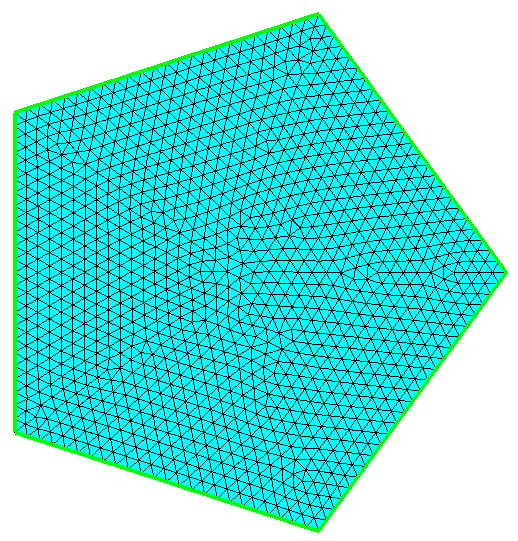
\includegraphics[width=100mm]{mesh}
\caption{The finite element mesh in ElmerGUI}\label{fg:pentagonmesh}
\end{center}
\end{figure}

After we have the mesh we start to go through the Model menu from the top to bottom. 
In the \texttt{Setup} we choose things related to the whole simulation such as file names, 
time stepping, constants etc.
The simulation is carried out in 2-dimensional Cartesian
coordinates and in steady-state (also used for eigenmodes). 
Only one steady-state iteration is needed as the case is linear. 
\ttbegin
Model
  Setup 
    Simulation Type = Steady state
    Steady state max. iter = 1
    Apply
\ttend

In the equation section we choose the relevant equations and parameters related to their solution. 
When defining Equations and Materials it is possible to assign to the bodies immediately, or to use mouse
selection to assign them later. In this case we have just one body and therefore its easier to assign 
the Equation and Material to it directly.

For the solver setting we need to activate the eigen mode computation. We also choose the 
direct umfpack solver which for small 2D problems often performs great.
\ttbegin
Model
  Equation
    Add 
      Name = Plate Equation
      Apply to bodies = 1
      Elastic Plates
        Active = on
        Edit Solver Settings 
          Solver Specific Options
            Eigen Analysis = on
            Eigen System Values = 10
          Linear System
            Direct = on
              Umfpack              
    Add  
    OK
\ttend        

The Material section includes all the material parameters.
They are divided into generic parameters which are direct properties of the material
without making any assumptions on the physical model, such as the mass. Other properties assume
a physical law, such heat Young's modulus. As our problem is academic in nature we choose some 
simple ideal parameters but data from material database could also be used instead.
\ttbegin
Model
  Material
    Add 
      Name = Ideal
      Apply to bodies = 1 
      General    
        Density = 1000.0
      Elastic Plates
        Youngs Modulus = 1e9
        Poisson ratio = 0.3
        Thickness = 0.001
        Tension = 0.0	
      Add
      OK
\ttend

A Body Force represents the right-hand-side of a equation i.e. external forces. In eigenmode analysis
no body forces are used. Nor are any Initial conditions required.

In this case all the boundaries are rigidly fixed we set all the components of the 
solution field to be zero. The 1st component is the displacement in the normal direction
while the 2nd and 3rd components are its derivatives in $x$ and $y$ directions.
\ttbegin
Model
  BoundaryCondition
    Add 
      Elastic Plates
        Deflection 1 = 0.0
        Deflection 2 = 0.0
        Deflection 3 = 0.0
      Name = Fixed
      Apply to boundaries = 1 2 3 4 5
      Add
      OK
\ttend   

For the execution 
ElmerSolver needs the mesh files and the command file. We have now basically defined
all the information for ElmerGUI to write the command file. After writing it we may also visually 
inspect the command file.
\ttbegin
Sif 
  Generate
  Edit -> look how your command file came out  
\ttend

Before we can execute the solver we should save the files in a directory. In saving the project all the
necessary files for restarting the case will be saved to the 
destination directory.
\ttbegin
File 
  Save Project
\ttend

After we have successfully saved the files we may start the solver
\ttbegin
Run
  Start solver
\ttend
A convergence view automatically pops up showing relative changes of each iteration.
In this case there is just one iteration and thus no curve appears.

\subsection*{Results}
The resulting eigenvalues are shown in table~\ref{tb:pentagonres}.
Note that some eigenmodes are degenerated but as the finite element mesh is not
perfectly symmetric there will be minor differences in the eigenvalues.

\begin{table}[h]
\caption{Ten lowest eigenvalues for the pentagon plate}
\label{tb:pentagonres}
\begin{center}
\begin{tabular}{ll} \hline
No & $\omega^2$ \\ \hline
1 & 18.9 \\
2,3 & 81.3 \\
4,5 & 214.5 \\
6   & 281.1 \\
7, 8 & 472.5 \\
9, 10 & 621.0 \\ \hline
\end{tabular}
\end{center}
\end{table}

Note: if you face problems in the solution phase and need to edit the setting, always remember to save
the project before execution.

To view the results we here start Paraview
\ttbegin
Run
  Paraview
\ttend
and select the 1st component of the \texttt{deflection} field
(confusingly named the x-component). 
If one chose for vtu output the mode \texttt{Eigen Analysis = True} then each file includes
one eigenmode. Then the eigenmodes may be treated as time steps. 
In figure~\ref{fg:pentagonpost} some of the lowest eigenmodes are depicted.
\begin{figure}
  \begin{center}
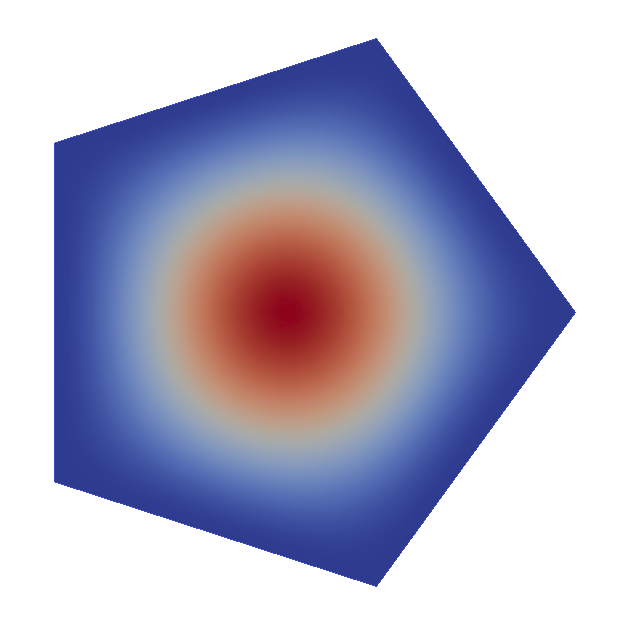
\includegraphics[width=40mm]{mode1}
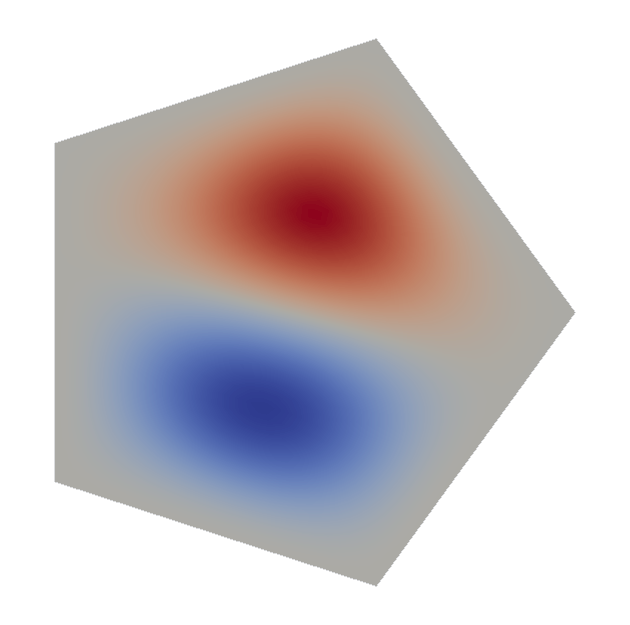
\includegraphics[width=40mm]{mode2}
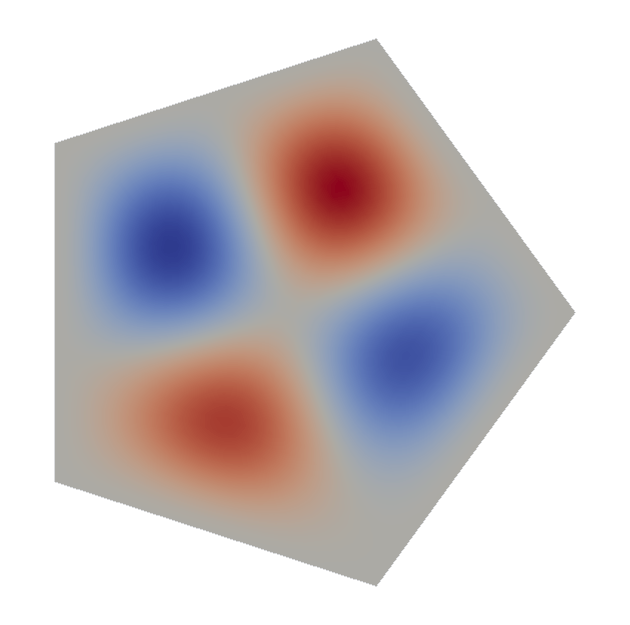
\includegraphics[width=40mm]{mode4} \\
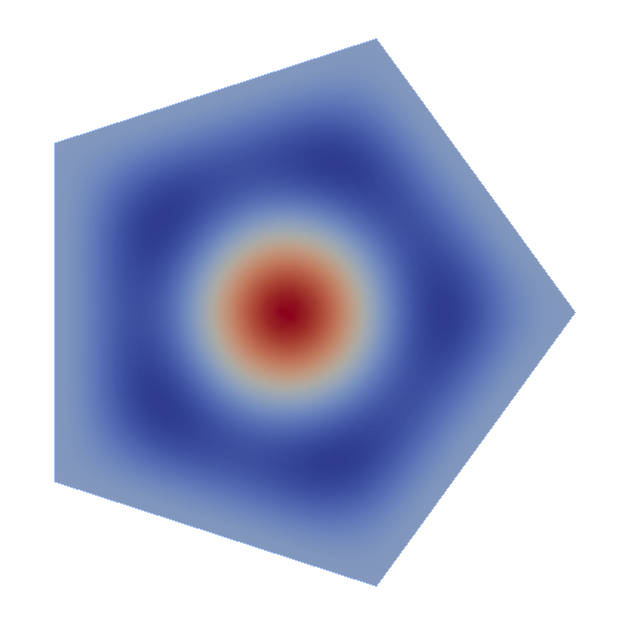
\includegraphics[width=40mm]{mode6}
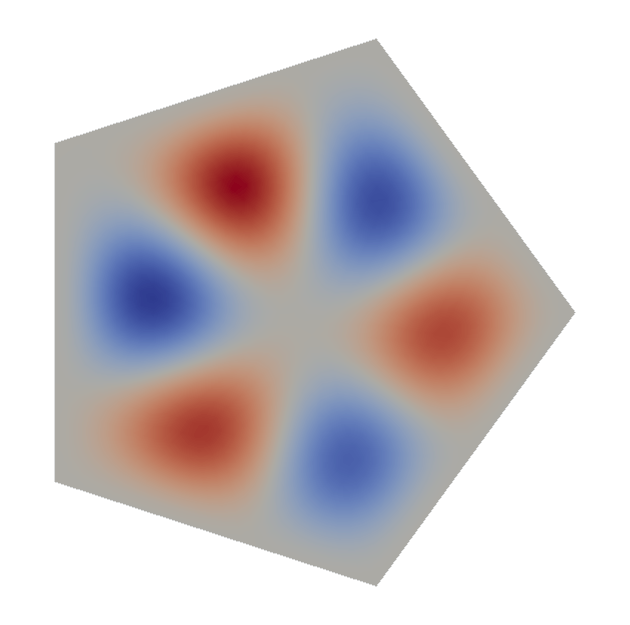
\includegraphics[width=40mm]{mode7}
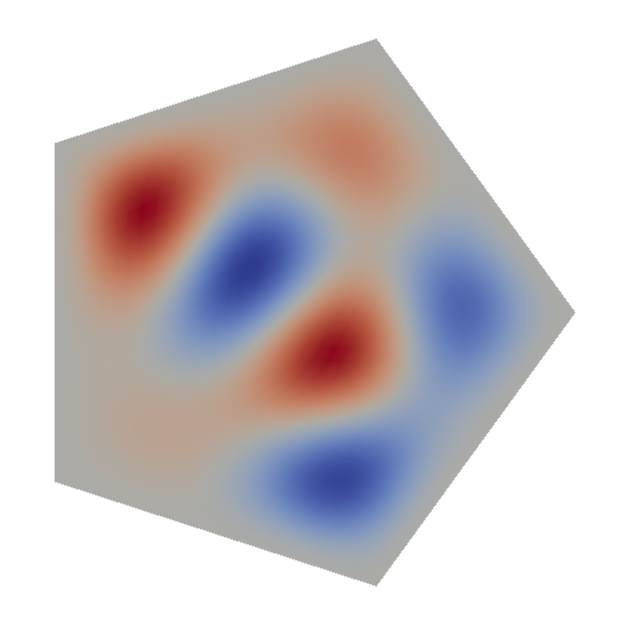
\includegraphics[width=40mm]{mode9}
\caption{The 1st, 2nd, 4th, 6th, 7th and 9th eigenmode of the plate. The displacement in the normal direction (first component) is shown.}
\label{fg:pentagonpost}
\end{center}
\end{figure}

\subsection*{Extra task}
You may test the effect of pre-stressing by altering the Tension material parameter.  

There are other similar geometries that you could use i.e. \texttt{hexagon.in2d}, \texttt{heptagon.in2d}, 
\texttt{octagon.in2d}.
When the number of vertices is increased the eigenvalues should slightly decrease. 



\hfill
\mbox{}






